\section{Experimental Setup}\label{sec:setup}
\textbf{Data.} Both datasets are real, public and cited: CIC-IoT2023~\cite{neto2023} (46 flow features; benign versus DDoS) and N-BaIoT~\cite{meidan2018} (115 features; benign versus Mirai/BASHLITE floods; scan classes excluded to stay in the DDoS scope). No synthetic data are used (Table~\ref{tab:datasets}). Each dataset is reduced to a seeded random pool and \emph{exact duplicate feature vectors are removed before any split} (\nv{dedup_removed:ciciot} of \nv{pool:ciciot} CIC-IoT2023 and \nv{dedup_removed:nbaiot} of \nv{pool:nbaiot} N-BaIoT pool rows). A corpus is a seeded stratified sample split 60/20/20 into train, validation and test (Fig.~\ref{fig:pipeline}).
\begin{table*}[t]
\centering
\caption{Datasets (real, public). The pool is a seeded random sample of the release; exact duplicates are removed before any split; the corpus is a seeded stratified sample split 60/20/20.}
\label{tab:datasets}
\scriptsize
\setlength{\tabcolsep}{2.4pt}
\begin{tabular}{p{1.0cm}p{3.6cm}p{2.6cm}p{0.7cm}p{0.9cm}p{0.9cm}p{1.6cm}p{2.5cm}p{0.5cm}}
\toprule
Dataset & Source / licence & Task / classes (release size) & Features & Pool rows & After de-dup & Corpus (seed 0) & Train/val/test & Clients \\
\midrule
CIC-IoT2023 & unb.ca/cic (mirror: HF lacg030175/CIC-IoT-2023-neto-full; CC-BY-4.0) \cite{neto2023} & benign vs 12 DDoS types (46.7M flows) & 46 & 809,836 & 772,037 & 200,000 (50\% attack) & 120,005/39,995/40,000 & 10 \\
N-BaIoT & UCI id 442, doi:10.24432/C5RC8J; CC BY 4.0 \cite{meidan2018} & benign vs 8 flood files (7.06M flows, 9 devices) & 115 & 300,000 & 227,775 & 136,939 (47\% attack) & 82,189/27,368/27,382 & 9 \\
\bottomrule
\end{tabular}
\end{table*}

\textbf{Clients.} CIC-IoT2023: $K{=}10$ clients with IID shards or Dirichlet label/attack-type skew~\cite{hsu2019}, $\alpha\in\{1.0,0.3,0.1\}$, over the benign class and twelve DDoS types. N-BaIoT: $K{=}9$, one client per device (natural skew), plus an IID control. Validation and test rows follow each client's training proportions; metrics are pooled over clients.

\textbf{Methods.} \emph{Central SVM/RF}~\cite{cortes1995,breiman2001} pool train-only preprocessed data. \emph{Senior} is the released pipeline (preprocessing fitted on all rows; independent \texttt{LinearSVC} per client; one weighted average); \emph{Senior (no leak)} fits it on training rows only. \emph{Local-prep FedAvg} is the naive alternative: each client runs the senior filters on its own rows, features chosen by at least half of the clients are kept, and each client standardises with its own statistics. \emph{FedStat-FS} is our method; \emph{+FedProx} adds the proximal term; \emph{FedAvg-MLP} trains a Keras 100-50 MLP on the same preprocessing. Ablations: A1 per-client scalers, A2 no selection (StatAvg-like), A3 one-shot cold-start averaging, A4 Pearson-only or LDA-only. All federated linear methods use $T{=}20$ rounds, $E{=}2$ local epochs, batch 64, step $\eta/(1+t)$; $\nu{=}0.01$, $\tau{=}0.2$, $k_L{=}20$ are shared.

\textbf{Fair tuning and statistics.} Every tuned method gets the same budget: random search, six trials from one random stream, scored by mean validation F1 over three corpora (seeds 0--2); the random forest uses its six-point grid. The test split is used once per run; final results use \nv{seeds} seeds (0--9) that change sample, split, partition and initialisation. Differences are paired over seeds, with two-sided Wilcoxon signed-rank $p$ values Holm-corrected over \nv{ntests} tests (smallest attainable raw $p$: \nv{minp}). Everything runs on CPU (Table~\ref{tab:setup}); TensorFlow trains every SGD-based detector.
\begin{table*}[t]
\centering
\caption{Experimental setup (CPU only) and tuning search spaces. Tuned values per dataset/condition are in results/tables/tuned\_hyperparameters.csv.}
\label{tab:setup}
\tiny
\setlength{\tabcolsep}{2.4pt}
\begin{tabular}{p{2.6cm}p{14.4cm}}
\toprule
Item & Setting \\
\midrule
Platform & Windows 11 Home (build 10.0.26200), native; AMD Ryzen 7 7435HS (8 cores / 16 threads); 23.7 GB RAM; CPU only \\
Software & Python 3.11.9, TensorFlow 2.21.0 / Keras 3.15.1, scikit-learn 1.9.1, NumPy 2.4.6, SciPy 1.17.1 \\
Splits, seeds & 60/20/20 stratified; 10 seeds (corpus sample, split, partition, initialisation) \\
Preprocessing & variance $\ge$ 0.01; Pearson $|\rho|>0.2$; LDA top-20; intersection; standardisation \\
FL protocol & T = 20 rounds, E = 2 local epochs, batch 64, plain SGD, lr/(1+r) decay, all clients each round \\
Tuning (all methods) & random search, 6 trials, same random stream; objective = mean validation F1 over the corpora of seeds 0--2; test never used \\
Search space: SVM family & lr $\in$ [0.005, 0.3] (log), C $\in$ [0.3, 100] (log), loss $\in$ \{hinge, sq. hinge\}; FedProx: $\mu_p$ $\in$ [1e-3, 1] (log) \\
Search space: MLP / RF & MLP: lr $\in$ [0.005, 0.3], L2 $\in$ [1e-5, 1e-2] (log); RF: trees $\in$ \{50,100\} $\times$ depth $\in$ \{10,20,30\} (6-point grid) \\
Senior baseline search & sklearn LinearSVC: C $\in$ [0.3, 100] (log), loss $\in$ \{hinge, sq. hinge\}, max\_iter 1000 \\
\bottomrule
\end{tabular}
\end{table*}
\begin{figure*}[t]
\centering
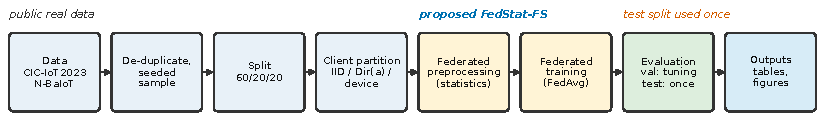
\includegraphics[width=\textwidth]{d2_pipeline_flowchart.pdf}
\caption{End-to-end pipeline: real public data are de-duplicated and split before any statistic is computed; validation drives tuning and the test split is used once.}
\label{fig:pipeline}
\end{figure*}
